% The two-tier workflow. Compiled standalone to workflow.pdf; uses the same Times
% face and the same palette as the plotted figures, and is sized so the paper
% includes it without rescaling.
%
% Colour carries the structure rather than decorating it: blue is the inner
% (placement) tier, which runs twice -- once per queued job and once per
% duplicate -- and orange is the outer (duplication) tier. Green marks the two
% loop tests; grey marks the entry and the exit.
\documentclass[border=3pt,11pt]{standalone}
\usepackage{times}
\usepackage{amsmath}
\usepackage{tikz}
\usetikzlibrary{arrows.meta, positioning, calc, fit, backgrounds, shapes.geometric}

% palette shared with the plotted figures (Okabe-Ito)
\definecolor{nblue}{HTML}{0072B2}
\definecolor{nverm}{HTML}{D55E00}
\definecolor{ngreen}{HTML}{009E73}
\definecolor{nink}{HTML}{1A1A1A}
\definecolor{nsoft}{HTML}{5A5A5A}
\definecolor{nrule}{HTML}{B0B0B0}

\begin{document}
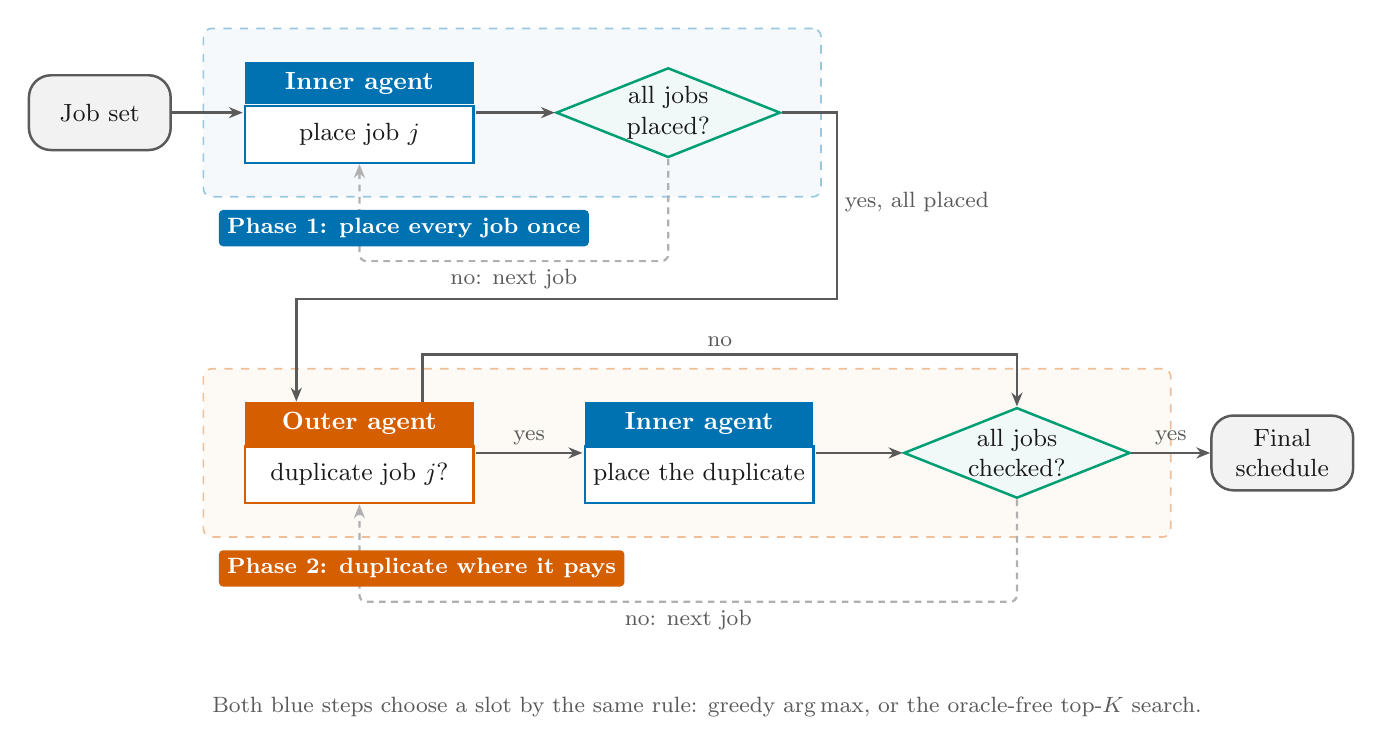
\begin{tikzpicture}[
  font=\small,
  >={Stealth[length=5pt, width=4pt]},
  % an agent is a titled card: colour-filled header over a white body
  header/.style  = {font=\small\bfseries, text=white, align=center,
                    minimum height=5.4mm, minimum width=29mm, inner sep=2pt},
  body/.style    = {font=\small, text=nink, align=center, fill=white,
                    minimum height=7.2mm, minimum width=29mm, inner sep=3pt},
  test/.style    = {diamond, aspect=2.5, draw=ngreen, line width=0.9pt,
                    fill=ngreen!6, align=center, inner sep=0.5pt,
                    text=nink, font=\small},
  terminal/.style= {draw=nsoft, line width=0.9pt, fill=black!5,
                    rounded corners=8pt, align=center, inner sep=4pt,
                    minimum height=9.5mm, minimum width=18mm, text=nink},
  flow/.style    = {->, draw=nsoft, line width=0.9pt},
  loop/.style    = {->, draw=nrule, line width=0.8pt, rounded corners=2.5pt,
                    dash pattern=on 2.4pt off 2pt},
  lbl/.style     = {font=\footnotesize, text=nsoft, inner sep=2.5pt},
  tab/.style     = {font=\footnotesize\bfseries, text=white, inner sep=3pt,
                    rounded corners=1.5pt},
]

% Agent card: #1 name, #2 placement, #3 colour, #4 title, #5 action.
% The placement option positions the *header*, so the card's centre sits half a
% body-height lower. To keep every connector orthogonal: position plain nodes
% relative to the card (<name>), and position one card relative to another
% card's header (<name>h) -- the cards share a geometry, so aligning headers
% aligns centres.
\newcommand{\agentcard}[5]{%
  \node[header, fill=#3, #2] (#1h) {#4};
  \node[body, draw=#3, line width=0.9pt, below=0pt of #1h.south,
        anchor=north] (#1b) {#5};
  \begin{scope}[on background layer]
    \node[draw=#3, line width=0.9pt, rounded corners=2pt,
          fit=(#1h)(#1b), inner sep=0pt] (#1) {};
  \end{scope}%
}

% ============================ row 1: place every job exactly once ===========
\agentcard{inner}{}{nblue}{Inner agent}{place job $j$}
\node[terminal, left=9mm of inner] (jobs) {Job set};
\node[test, right=10mm of inner] (placed) {all jobs\\placed?};

\draw[flow] (jobs)  -- (inner);
\draw[flow] (inner) -- (placed);
\draw[loop] (placed.south) -- ++(0,-13mm)
            -| node[lbl, pos=0.25, below] {no: next job} (innerb.south);

% ============================ row 2: decide duplication per job =============
\agentcard{outer}{below=30mm of inner, anchor=north}{nverm}%
          {Outer agent}{duplicate job $j$?}
\agentcard{dup}{right=14mm of outerh, anchor=west}{nblue}%
          {Inner agent}{place the duplicate}
\node[test, right=11mm of dup] (checked) {all jobs\\checked?};
\node[terminal, right=10mm of checked] (sched) {Final\\schedule};

\draw[flow] (outer) -- node[lbl, above] {yes} (dup);
\draw[flow] (dup)   -- (checked);
\draw[flow] (checked) -- node[lbl, above] {yes} (sched);
% "no" skips the duplicate placement entirely, leaving from the right of the card
\coordinate (noout) at ($(outerh.north)!0.55!(outerh.north east)$);
\draw[flow] (noout) -- ++(0,6mm) -| node[lbl, pos=0.25, above] {no}
            ($(checked.north)+(0,6mm)$) -- (checked.north);
\draw[loop] (checked.south) -- ++(0,-13mm)
            -| node[lbl, pos=0.25, below] {no: next job} (outerb.south);

% the phases are joined by a single wrap from the end of row 1
\coordinate (wrapin) at ($(outerh.north)!0.55!(outerh.north west)$);
\draw[flow] (placed.east) -- ++(7mm,0)
            |- node[lbl, pos=0.24, right] {yes, all placed}
            ($(wrapin)+(0,13mm)$) -| (wrapin);

% ================================================================ framing ===
\begin{scope}[on background layer]
  \node[fit=(inner)(placed), draw=nblue!40, line width=0.6pt, dashed,
        rounded corners=3pt, inner xsep=5mm, inner ysep=4mm,
        fill=nblue!4] (p1) {};
  \node[fit=(outer)(dup)(checked), draw=nverm!40, line width=0.6pt, dashed,
        rounded corners=3pt, inner xsep=5mm, inner ysep=4mm,
        fill=nverm!4] (p2) {};
\end{scope}
\node[tab, fill=nblue, anchor=north west] at ($(p1.south west)+(2mm,-1.5mm)$)
     {Phase 1: place every job once};
\node[tab, fill=nverm, anchor=north west] at ($(p2.south west)+(2mm,-1.5mm)$)
     {Phase 2: duplicate where it pays};

% ------------------------------------------------------- one line of context
\node[font=\footnotesize, text=nsoft, align=left, anchor=north west]
     at ($(p2.south west)+(0mm,-19mm)$)
     {Both blue steps choose a slot by the same rule: greedy $\arg\max$, or the
      oracle-free top-$K$ search.};

\end{tikzpicture}
\end{document}
